\chapter{Process Diagram grammar}
\label{chp:grammar}

\section{Overview}

In this chapter, we describe how the glyphs of SBGN can be combined
to make a valid SBGN diagram. To do this, we must at the very least
define what glyphs can be connected to each other. This is called
syntax. Next, we must define rules over and above connection rules,
such as whether duplicate symbols are permitted. In addition, we must define what the notation ``means'' --- how does it represent a biological pathway? This is semantics, and it is essential if a reader is to understand a SBGN diagram without external help, and a writer is to create one that reflects his understanding of a biological system.

In this section we start off by describing the concepts of the
\PD{} notation. Next a detailed description of the syntax is provided
followed by a description of the syntactic rules of the notation.

\section{Concepts}

The SBGN \PD{} is more than a collection of symbols. It is a
visual language that uses specific abstractions to describe the
biological processes that make up a quantitative model, a signalling pathway or a metabolic network. This abstraction is the
semantics of SBGN, and to describe it requires more than a definition
of the symbols and syntax of the language. We first need to define the
abstractions we are using.

The \PD{} in SBGN describes biological processes involving biological entities. An \glyph{Entity pool node} (\sect{EPNs}), such as a molecule, is converted into other \glyph{EPNs} via a process. 

It may be convenient to think of a SBGN \PD{} as describing the
flow of a fluid. In this analogy, each \glyph{EPN} represents a
tank of fluid, which may be emptied via a pipe (the consumption arc, \sect{consumption}) 
that is connected to a valve (the process node, \sect{PNs}), which in turn is
connected to other pipes (the production arcs, \sect{production}) that fill other tanks
(\glyph{EPNs}). A valve can be
controlled in relation to the amount of fluid in another tank.  This
precise nature of the relationship between valve opening and amount of
fluid determines the nature of the modulation.

%%  In SBGN modulation takes 3 forms:

%% \begin{enumerate}
%% \item The rate of fluid flow through the value is opened is related to the amount of fluid in the modulating tank (modulation arc).
%% \item The rate is directly related to the fluid level in the modulating tank (activation arc).
%% \item The rate is inversely related to the fluid level in the modulating tank (inhibition arc; note that a catalysis arc is identical to this).
%% \end{enumerate}

%% A more subtle form of modulatory control is exhibited by special
%% ```logic'' valves that open based on boolean logic (Logic Gates).
%% These are as follows:

%% \begin{description}
%% \item[AND] The valve has more than one input pipe. If water flows in both pipes then the value opens and lets water flow into its output pipe.
%% \item[OR] This is equivalent to two pipes that flow into one. Fluid from two or more input pipes is directed to the output pipe.
%% \item[NOT] This value must work in conjunction with another valve and
%%   has one input and one output pipe. If fluid flows into the valve
%%   then nothing flows out of it and if there is no flow into it there
%%   is flow out of it.
%% \end{description}

%% The input pipe to a logic valve is in turn connected to a
%% ``pressure-dependent'' value (Existence Arc). This valve only opens at
%% a specified pressure and so it allows us to determine a threshold
%% above which water can flow to the logic valve. This is important as it
%% allows us to convert an analogue value (fluid pressure or in the case
%% of SBGN the concentration of a chemical Entity Pool Node) into a digital true
%% or false value required by Boolean logic.

Finally, the system needs a source of fluid from one or
more external sources (\glyph{source}, section \sect{sourceSink}) and somewhere for it to drain away (the
\glyph{sink}).

% This analogy can equally apply to an electronic circuit.% where the
%valves may be transistors, the Entity Pool Node capacitors, sources the cathode
%of a battery and an earth as the sink.

\section{The conceptual model}

In order to formalize the conceptual representation described above
and the semantic rules that we will describe later, we have developed a UML
Domain Object Model of SBGN\@. This defines what would otherwise be
vaguely defined in the SBGN specification, and enables us to define
clearly what is a valid SBGN diagram.

The model is separated into two layers. The Visual Layer
(\fig{sbgn_visual}) directly maps to the glyphs used to
visualise SBGN and reflects the syntax of the notation. The Conceptual
Layer describes what is ``meant'' by the visual SBGN representation
(\fig{sbgn_conceptual}). It is important in defining
concepts such as Entity types and state variables that are implicit in the Visual Layer.

 \begin{landscape}
\begin{figure}[p]
\begin{center}
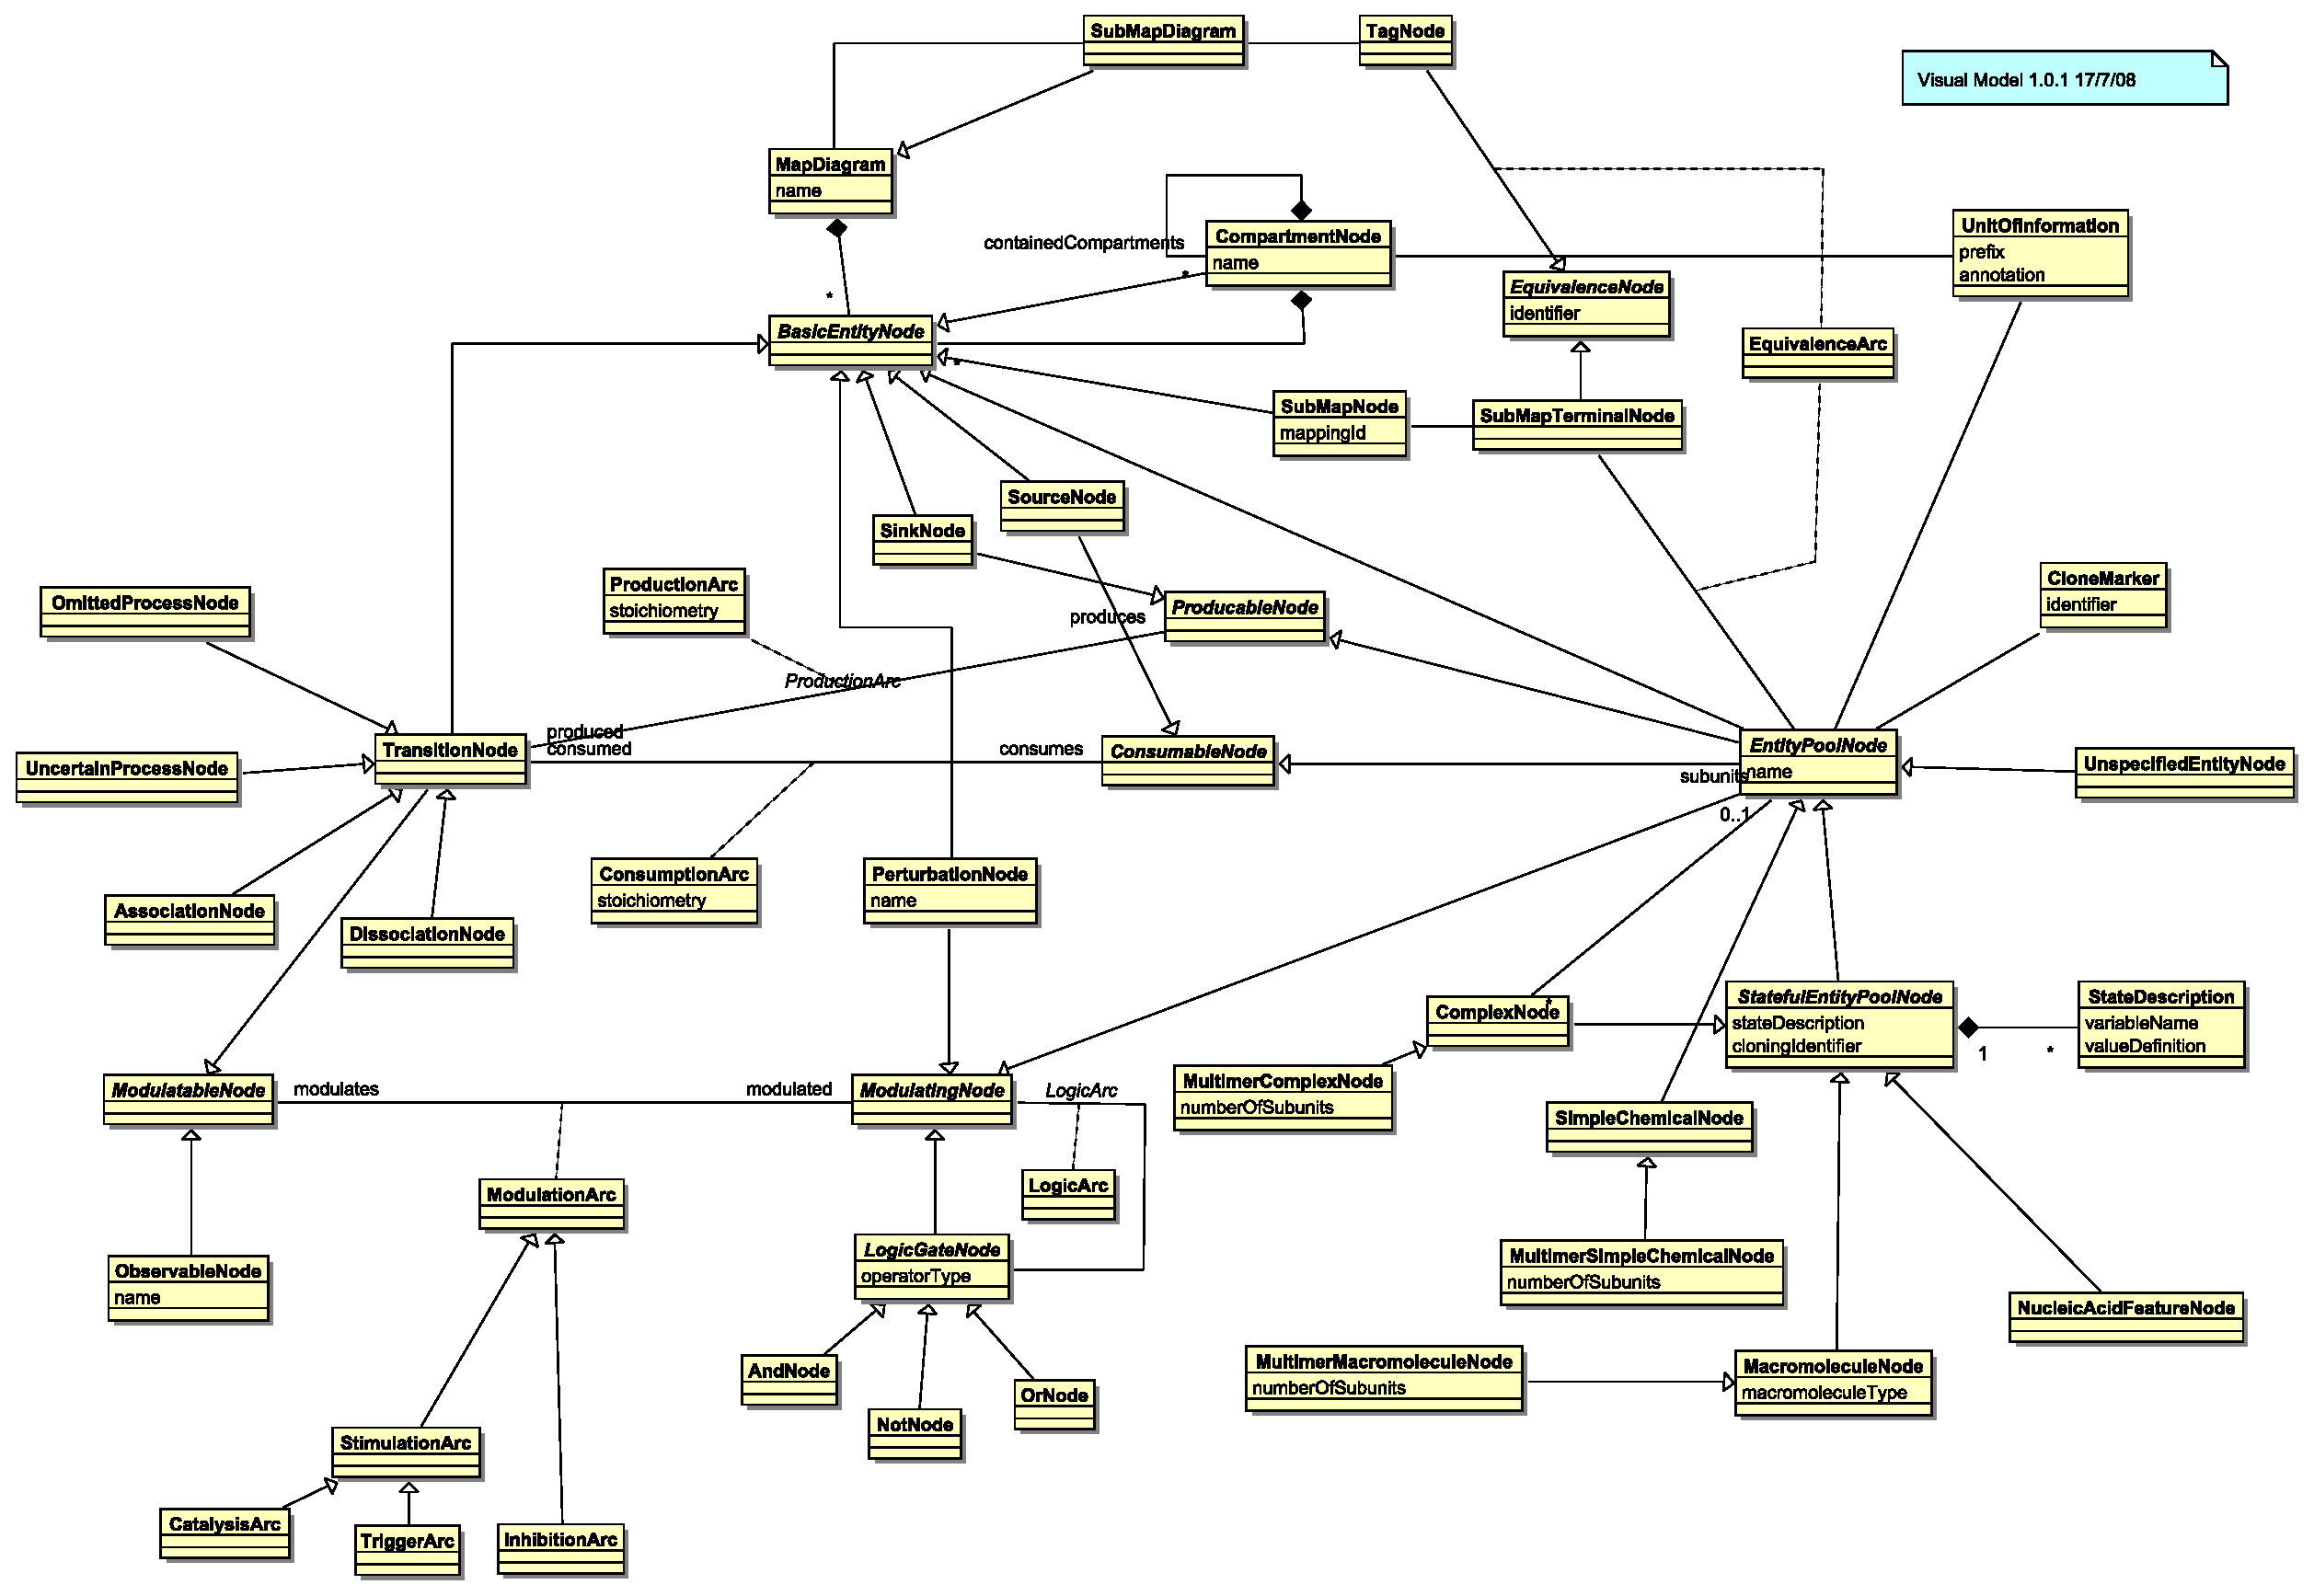
\includegraphics[width=0.85\linewidth]{images/sbgn_visual}
\caption{UML model of SBGN visual representation. Class names shown in italics are abstract classes and do not correspond to a glyph. Classes in non-italicised script with the suffixes ``Node'' and ``Arc'' correspond to node and arc glyphs respectively.}
\label{fig:sbgn_visual}
\end{center}
\end{figure}

\begin{figure}[p]
\begin{center}
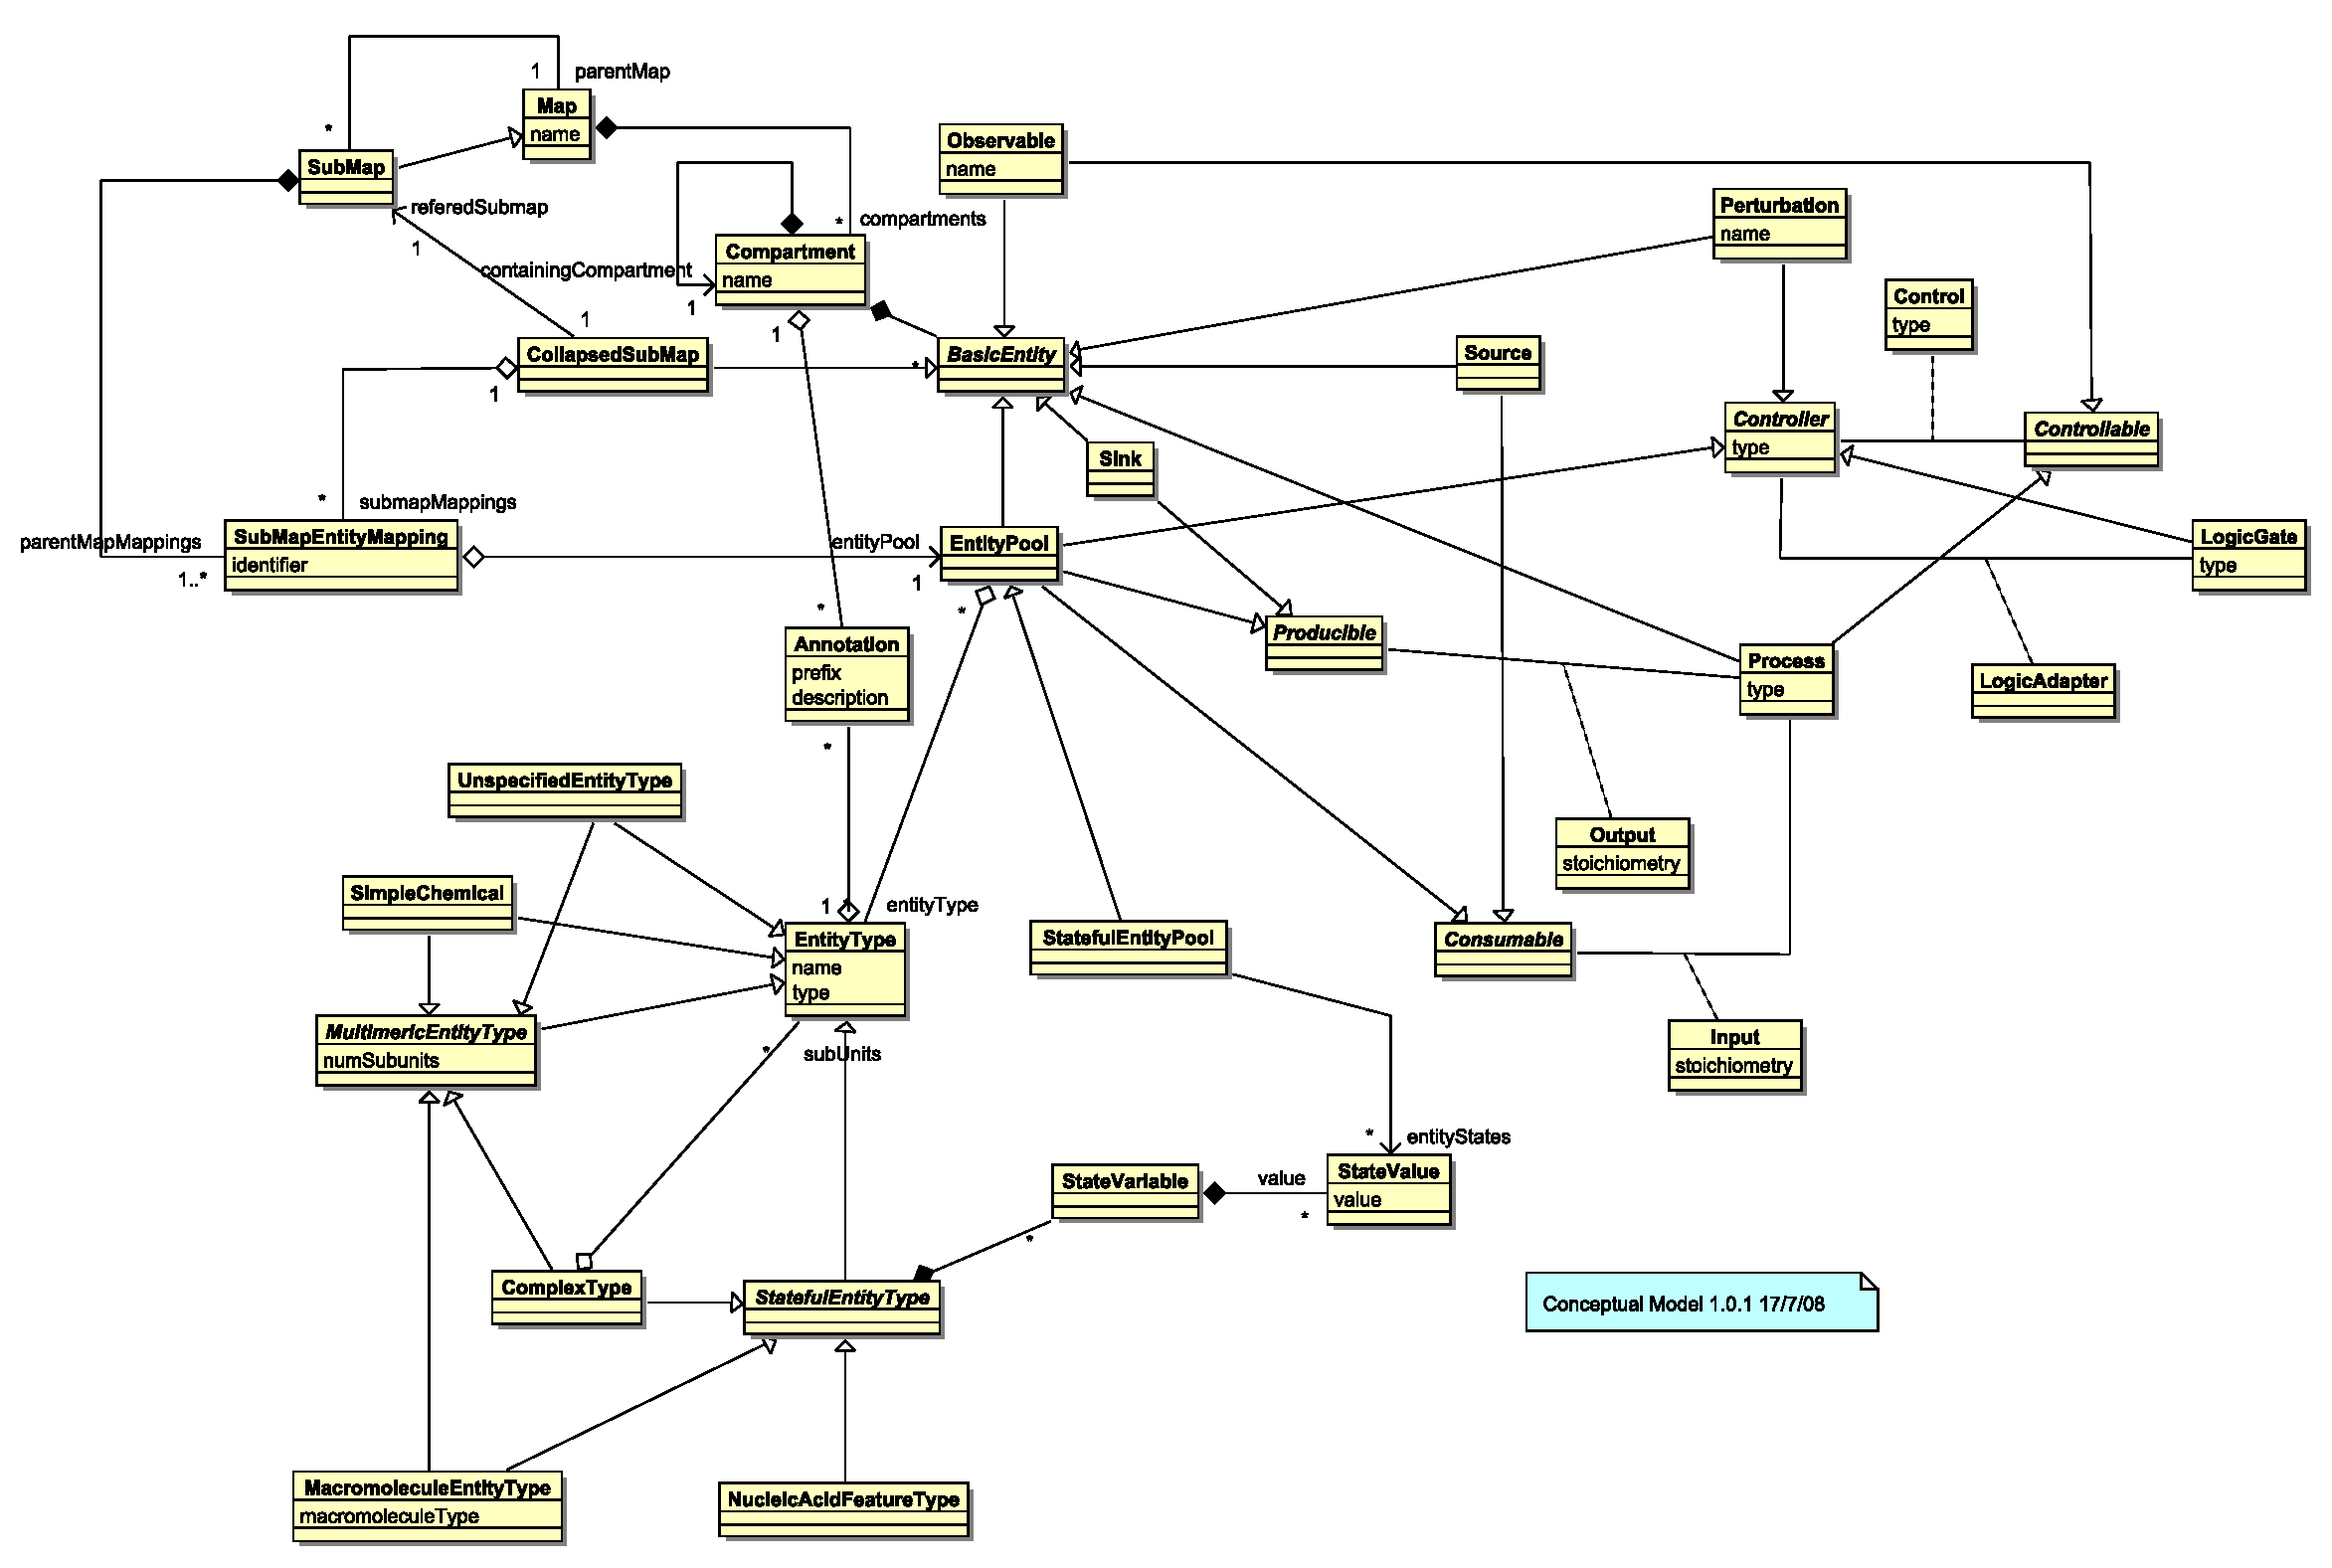
\includegraphics[width=0.85\linewidth]{images/sbgn_conceptual}
\caption{UML model of SBGN conceptual representation. The main difference between visual and conceptual representaions is that the conceptual model is non-redundant with only one instance of an EntityPool with a given identity. Each class has a mapping back to the Visual Layer.}
\label{fig:sbgn_conceptual}
\end{center}
\end{figure}
\end{landscape}
The Classes shown in the UML model are described in more detail in the
tables below. In particular the tables define the properties that
uniquely identify each component of the notation. This is important in
defining the rules for duplication and the submap interface later.

\newlength{\commlen}
\setlength{\commlen}{6cm}
\begin{landscape}
\begin{center}
\begin{scriptsize}
\tablefirsthead{\hline\multicolumn{5}{|c|}{Visual Layer Data Dictionary}\\\hline
 Name & \multicolumn{2}{|c|}{Attributes} & Glyph & Comment\\\cline{2-3}
 & Name & Description & & \\\hline}
\tablehead{\hline
\multicolumn{5}{|l|}{\small\sl continued from previous page}\\\hline
Name & \multicolumn{2}{|c|}{Attributes} & Glyph & Comment\\\cline{2-3}
 & Name & Description & & \\\hline\hline}
\tabletail{\hline
\multicolumn{5}{|r|}{\small\sl continued on next page}\\
\hline}
\tablelasttail{\hline}

\topcaption{A data dictionary for the Visual Layer of the SBGN
  Conceptual Model. Attributes that uniquely identify a class are
  followed by (I) and required attributes by (R): it is implied that
  identifying attributes are also required. The default cardinality of
  an attribute is one (or zero or one if it is not required) unless
  otherwise specified. A standard notation for cardinality is used,
  for example \{0 \ldots *\} should be read zero, one or many. The Glyph
  column states the Glyph the class maps to, unless the class is
  purely conceptual and so defined as Abstract.}


\begin{supertabular}{|p{3cm}|p{4cm}|p{5.5cm}|p{2.5cm}|p{\commlen}|}\hline
%
MapDiagram & name (I) & Name of the map. & N/A & The diagram is the visualisation of a SBGN map.\\\hline
%
SubmapDiagram & mainMapName (I) & Name of the main map this is a sub-map of.& N/A & \multirow{2}{\commlen}{A SBGN diagram used to define a SBGN submap}\\
& name (I) & Name of the sub-map. & & \\\hline
%
BasicEntity\-Node & & & Abstract & The most fundamental node type. Any node that can be drawn on a MapDiagram inherits from this.\\\hline
%
ConsumableNode & & & Abstract & Nodes that can be consumed and are connected at the start of a consumption arc.\\\hline
%
ProducableNode & & & Abstract & Nodes that can produced and are linked to the end of a production arc.\\\hline
%
ModulatableNode & modulatingNodes (I) \{0 \ldots *\} & Any number of
nodes that modulate this one.& Abstract & Nodes representing a process
that can be modulated and so are linked to the end of a modulation arc.\\\hline
%
ModulatingNode & & & Abstract & Nodes that can modulate modulatable nodes. They are linked to the origin of a modulating arc.\\\hline
%
CompartmentNode & name (I) & Name of compartment being defined. At present the name of the compartment is not restricted, i.e.\, a controlled vocabulary is not used. & Compartment & \\
& unitsOfInformation \{0 \ldots *\} & any number of Units of Information. & &\\\hline
%
EntityPoolNode (EPN) & name (I) & The name of the entity. & Abstract & \multirow{3}{\commlen}{Nodes that inherit from this type are generally chemical species that can be produced, consumed or transformed in chemical processes. It refers to a population (or pool) of such species.} \\
 & compartment (I) & If no compartment is specified then this is implicitly defined as the ``default'' compartment. & & \\
& unitsOfInformation \{0 \ldots *\} & Any number of Units of Information. & &\\\hline
%
StatefulEntity\-Pool\-Node & As EPN & & Abstract & \multirow{2}{\commlen}{All EPN that inherit from this class may have state variables assigned to them.}\\
& stateDescriptions (I) \{0 \ldots *\} & Any number of StateDescriptions associated with this EPN. & &\\\hline
%
SimpleChemical\-Node & As EPN & & SimpleChemical & \\\hline
%
Unspecified\-Entity\-Node & As EPN &  & UnspecifiedEntity & \\\hline
%
SourceNode & &  & Source/Sink & The SourceNode can only be associated with \emph{one} consumption arc. Note that this shares the same Glyph as SinkNode.\\\hline
%
SinkNode & & & Source/Sink & The SinkNode can only be associated with \emph{one} production arc. Note that this shares the same Glyph as SourceNode.\\\hline
%
ObservableNode & name (I) & Name of the observable. & Observable & \\\hline
%
PerturbationNode & name (I) & Name of the perturbation. & Perturbation & \\\hline
%
MacromoleculeNode & As StatefulEntityPoolNode & & Macromolecule & \multirow{2}{\commlen}{} \\
 & macromoleculeType (I) & The type of the macromolecule. Currently there are no constraints on permitted types. & & \\\hline
%
Nucleic\-Acid\-Feature\-Node & As StatefulEntityPoolNode & & Nucleic\-Acid\-Feature & \\\hline
%
ComplexNode & As StatefulEntityPoolNode & & Complex & \multirow{3}{\commlen}{} \\
 & subunits \{0 \ldots *\} & A list of EPNs that together compose the complex. & & \\
 & subunitStates (I) \{0 \ldots *\} & The set of state descriptions of any Subunits that are StatefulEntityPoolNodes. & & \\\hline
%
Multimer\-Macromolecule\-Node & As MacromoleculeNode & & Multimer\-Macromolecule & \multirow{2}{\commlen}{Note that all sub-units have the \emph{same} StateDescription values.} \\
 & numberOfSubunits (I) & The number of identical sub-units of this macromolecule. & & \\\hline
%
MultimerSimple\-Chemical\-Node & As SimpleChemicalNode & & MultimerSimple\-Chemical & \multirow{2}{\commlen}{} \\
& numberOfSubunits (I) & The number of identical sub-units of this simple chemical. & & \\\hline
%
MultimerComplex\-Node & As ComplexNode & & MultimerComplex & \multirow{2}{\commlen}{Note that all sub-units have the \emph{same} StateDescription values.}\\
 & numberOfSubunits (I) & The number of identical sub-units of this complex. & & \\\hline
%
UnitOfInformation & owningEPN (I) & Identity of the owning EntityPoolNode (not displayed, but implied by ``ownership'' of the glyph). & Unit Of Information & \multirow{2}{\commlen}{} \\
& prefix & Prefix (I) & & \\
& annotation & Annotation (R) & & \\\hline
%
StateDescription & owningStatefulEPN & Identity of the owning Stateful\-Entity\-Pool\-Node (not displayed, but implied by ``ownership'' of the glyph). & State Variables & \multirow{3}{\commlen}{} \\
 & variable & The name (identification) of the ``state variable'' glyph associated a StatefulEntityPoolNode. & & \\
 & value &  The definition of a value for the given variable. & & \\\hline
%
ProcessNode & As ModulatableNode & & Process & \multirow{3}{\commlen}{}\\
 & producableNodes (I) \{1 \ldots *\} & The ProducableNodes linked to the process by a ProductionArc. & & \\
 & consumableNodes (I) \{1 \ldots *\} & The ConsumableNodes linked to the process by a ConsumptionArc. & & \\\hline
%
OmittedProcess\-Node & As Process Node & & Omitted Process &\\\hline
%
UncertainProcess\-Node & As Process Node & & Uncertain Process & \\\hline
%
Association\-Node & As Process Node & & Association & \\\hline
%
Dissociation\-Node & As Process Node & & Dissociation& \\\hline
%
LogicGateNode & gateType (I) & The type of boolean gate. Currently one of OR, AND, NOT. & Abstract & \multirow{3}{\commlen}{Not a glyph but a placeholder for the common behaviour of all logic gates.}\\
 & modulatingNodes (I) & The modulating nodes that are the input the Boolean logic operator. They must be linked via a LogicArc. & & \\
 & modulatedNode (I) & A ModulatableNode connected via a Modulation\-Arc or another Logic\-Gate\-Node connected via a LogicArc. & & \\\hline
%
ANDNode & As LogicGateNode & & And & \\\hline
%
ORNode & As LogicGateNode & & Or & \\\hline
%
NOTNode & As LogicGateNode & & Not & \\\hline
%
SubMapNode & subMapName (I) & The name of the sub-map it is defining. & Submap & \multirow{2}{\commlen}{} \\
 & compartment (R) & If no compartment is specified then this is implicitly defined as the ``default'' compartment. & & \\\hline
%
TagNode & subMapName (I) & Name of submap that owns tag. & Tag & \\
& identifier (I) & A name that uniquely identifies the tag on the submap. & & \\\hline
%
SubMapTerminalNode & subMapName (I) & Name of submap that owns labeled terminal. & SubMapTerminal & \\
& identifier (I) & A name that uniquely identifies the terminal on the submap. & & \\\hline
%
ProductionArc & processNode (I) & The ProcessNode that this is the output of. & Production & \multirow{2}{\commlen}{It is assumed that the arc is unidirectional.} \\
 & producableNode (I) & The ProducableNode that is the product of the process. & & \\\hline
%
ConsumptionArc & consumableNode (I) & The ConsumableNode that is the input to the process. & Consumption & It is assumed that the arc is unidirectional.\\
 & processNode (I) & The ProcessNode that this is the input to. & & \\\hline
%
ModulationArc & modulatingNode (I) & The ModulatingNode that is the origin of this link. & Modulation & \multirow{2}{\commlen}{} \\
 & modulatedNode (I) & The ModulatableNode that is controlled (modulated) by this arc. & & \\\hline
%
StimulationArc & As ModulationArc & & Stimulation & \\\hline
%
CatalysisArc & As ModulatioArc & & Catalysis & \\\hline
%
InhibitionArc & As ModulationArc & & Inhibition & \\\hline
%
Necessary StimulationArc & As ModulationArc & & Inhibition & \\\hline
%
LogicArc & modulatingNode (I) & The ModulatingNode that is the origin of this link. & LogicArc & \multirow{3}{\commlen}{Conceptually this class can be thought of as converting a continuous input (the population of the EntityPool) into a discrete Boolean output (True or False).} \\
 &  &  & & \\
 & logicGate (I) & The logicGateNode that is the target of this link. & & \\\hline
%
% TagArc & tag (I) & The tag assigned to with the EPN. & Tag & \multirow{2}{\commlen}{} \\
%  & taggedEPN (I) & The EPN assigned to the tag. & & \\\hline
EquivalenceArc & Tag (I) & The tag assigned to with the EPN. & Tag & \multirow{2}{\commlen}{} \\
 & EPN (I) & The EPN assigned to the tag. & & \\\hline
%
\end{supertabular}
\end{scriptsize}
\end{center}

\newlength{\mappinglen}
\setlength{\mappinglen}{3.5cm}
\newlength{\desclen}
\setlength{\desclen}{5.5cm}
\begin{center}
\begin{scriptsize}
\tablefirsthead{\hline\multicolumn{5}{|c|}{Conceptual Layer Data Dictionary}\\\hline
Name & \multicolumn{2}{|c|}{Attributes} & Description & Mapping to Visual Layer\\\cline{2-3}
 & Name & Description & & \\\hline}
\tablehead{\hline
\multicolumn{5}{|l|}{\small\sl continued from previous page}\\
\hline\hline
Name & \multicolumn{2}{|c|}{Attributes} & Description & Visual Mapping\\\cline{2-3}
 & Name & Description & & \\\hline\hline}
\tabletail{\hline
\multicolumn{5}{|r|}{\small\sl continued on next page}\\
\hline}
\tablelasttail{\hline}

\topcaption{A data dictionary for the Conceptual Layer of the SBGN
  Model. Attributes that uniquely identify a class are
  followed by (I) and required attributes by (R): it is implied that
  identifying attributes are also required. The default cardinality of
  an attribute is one (or zero or one if it is not required) unless
  otherwise specified. A standard notation for cardinality is used,
  for example \{0 \ldots *\} should be read zero, one or many. A mapping to a class in the Visual Layer is provided where appropriate.}

\begin{supertabular}{|p{3cm}|p{4cm}|p{6cm}|p{\desclen}|p{\mappinglen}|}\hline
%
Map & name (I) & A name or identifier for the map. & The biological pathway that is represented by the SBGN diagram. & MapDiagram\\\hline
%
SubMap & name (I) & The name of the submap. &  & SubMapDiagram\\
 & mainMapName (I) & The name of the map that refers to this submap. & & \\\hline
%
Compartment & name (I) & The name of the compartment. & & CompartmentNode\\\hline
%  & containingCompartment & The compartment that contains this compartment, if any. & & \\\hline
%
BasicEntity & & & Root class of all Entities that can be contained by a Compartment. & BasicEntityNode \\\hline
%
Controller & & & Something that can control a Controllable. & ModulatingNode \\\hline
%
Controllable & & & Something that can be controlled by a Controller & ModulatableNode \\\hline
%
Producible & & & Something that can be produced by a process. & ProducibleNode \\\hline
%
Consumable & & & Something that can be consumed by a process. & ConsumableNode \\\hline
%
EntityType & Name (I) & The name of the EntityType. & \multirow{2}{\desclen}{This is the type of the EntityPool.} & \multirow{2}{\mappinglen}{No direct maps to the visual layer. It is an implied attribute of the EntityPoolNode.}\\
& type (I) &  Type of the Entity. One of: SimpleChemical, UnspeciedEntity, Complex, Macromolecule, and Nucleic\-Acid\-Feature. & & \\
 & annotations \{0 \ldots *\} & Annotation must be associated with the type and be general to all Entity Pool Node. If it were associated with the Species then this would be synonymous with a state description. & & \\\hline
%
Multimeric\-Entity\-Type & As EntityType & & An Entity that can form homo-multimeric complexes. All copies share the same attributes. & \\
 & cardinality (I) & The number of subunits in the monomer. & & \\\hline
%
Stateful\-Entity\-Type & As EntityType & & An EntityType that can have state variables associated with it. & \\
 & stateVariables \{ 0 \ldots * \} & & & \\\hline
%
Complex\-Entity\-Type & As Stateful\-Entity\-Type & & & \multirow{3}{\mappinglen}{Implicitly defined by a ComplexNode.} \\
 & cardinality (I) & from MultimericEntityType. & & \\
 & subunits \{ 0 \ldots * \} & The set of EntityTypes that the complex composed of. & & \\\hline
%
Macromolecule\-Entity\-Type & macromoleculeType (I) &  The type of the macromolecule. The permitted type names are not constrained as yet. Suggest types are protein, mRNA, miRNA, tRNA, rRNA, DNA, polysaccaride. See also controlled vocabularies for material type \ref{sec:material-types-cv} and conceptual type \ref{sec:conceptual-types-cv} & & Implicitly defined by a Macromolecule\-Node and Multimer\-Macromolecule\-Node\\\hline
%
StateVariable & name (I) & The name of the state variable. & \multirow{2}{\desclen}{The state variable is assigned to a StatefulEntityType and can have one or more values assigned to it when used in a StatefulEntityPool.} & \multirow{2}{\mappinglen}{The name of a State\-Description.} \\[20pt]
 & & & & \\
%  & domainValues \{1 \ldots * \} & The domain of the StateVariable, i.e. the set of possible values it can hold. This is required because an Stateful\-Entity\-Pool is assigned a set of state values for a given StateVariable. & & \\
 \hline
%
StateValue & value (I) & The value of the state. & A value that can be assigned to a state variable. & The value string or ``regexp'' used in the State\-Description.\\\hline
%
EntityPool & entityType (I) & The EntityType of the pool. & An instantiation of an EntityType. & EntityPoolNode\\\hline
%
StatefulEntity\-Pool & As EntityPool & & & \multirow{2}{\mappinglen}{Stateful\-Entity\-Pool\-Node} \\
 & stateValueSets \{1 \ldots * \} &  A set of state values assigned to a the State\-Variables of the associated Stateful\-Entity\-Type. & & \\\hline
%
ComplexEntityPool & As StatefulEntity & & \multirow{3}{\desclen}{The instantiation of a complex that is defined by it's own state and the states of its subunits.} & ComplexNode \\
 & subunitValues (I) \{0 \ldots * \} &  The set of StateValues for all subunits. & & \\
 & & & & \\\hline
%
Annotation & prefix (I) & A classifier for the annotation. & & UnitOfInformation\\
 & annotation & Annotation that is associated with a Entity\-Type or Compartment. & & \\\hline
%
Process & processType (I) &  One of: Unspecified, Dissociation, Association, Omitted Process, Uncertain Process. & & The type is specified by the type of Glyph used: Process\-Node, Dissociation\-Node, Association\-Node, Omitted\-Process\-Node, Uncertain\-Process\-Node.\\\hline
%
Output & process (I) & The process that this is the output of. & & ProductionArc \\
 & product (I) & The EPN that is the product of the process. & & \\\hline
%
Input & substrate (I) & The EPN that is the input to the process. & & ConsumptionArc \\
 & process (I) & The process that this is the input of. & & \\\hline
%
Control & type (R) & The type of the control. One of Modulation, Stimulation, Inhibition, Necessary Stimulation, Catalysis or LogicGate. & & ModulationArc \\\hline
%
LogicGate & type (R) & The type of LogicGate. One of AND, OR, NOT. & & LogicGateNode \\\hline
%
LogicAdapter & & & The LogicGate takes a set of Boolean inputs (T or F) from an EntityPool which is a non-Boolean quantity. Conceptually, the adapter converts the continuous quantity into a discrete Boolean quantity. & LogicArc \\\hline
%
Perturbation & name & Name of the perturbation. & & PerturbationNode \\\hline
%
Observable & name & Name of the observable. & & ObservableNode \\\hline
%
Source & & & & SourceNode \\\hline
%
Sink & & & & SinkNode \\\hline
%
Collapsed\-Sub\-Map & referredSubMap (I) & Submap that this refers too. & The submap is ``collapsed'' down to this element, which acts as a placeholder for the submap. & SubMapNode \\\hline
%
SubMap\-Entity\-Mapping & identifier (I) & Identifier in Visual layer to link Entity\-Pool\-Nodes in the main map and submap. & \multirow{3}{\desclen}{A definition of the mapping between the submap and main map for a single EntityPool.} & \multirow{3}{\mappinglen}{SubMap\-Terminal\-Node and Tag\-Node}\\
 & entityPool (R) & The EntityPool node that is mapped between the submap and the main map. & & \\\hline
%
\end{supertabular}
\end{scriptsize}
\end{center}
\end{landscape}

\section{Syntax}

The syntax of the SBGN \PDl is defined in the form of an incidence matrix. An incidence matrix has arcs as rows and nodes as columns. Each element of the matrix represents the role of an arc in connection to a node. Source (S) means that the arc can begin at that node. Target (T) indicates that the arc can end at that node. Numbers in parenthesis represent the maximum number of arcs of a particular type to have this specific connection role with the node. Empty cells means the arc is not able to connect to the node.

\subsection{Node connectivity}

\begin{center}
\begin{tabular}{||c|c|c|c|c|c|c|c|c|c|c|c|c||}
\hline
\hline
\raisebox{20pt}{$Arc \backslash EPN$} &\vglyph{macromolecule} & \vglyph{simple chemical} & 
\vglyph{unspecified entity} &  \vglyph{multimer} & \vglyph{complex} & 
\vglyph{nucleic acid feature}& \vglyph{tag} & \vglyph{submap terminal} & \vglyph{empty set} & 
\vglyph{perturbing agent} &  \vglyph{submap}\\ \hline 
\glyph{consumption}      & S & S & S & S & S & S &   & & S(1) &  & \\ \hline 
\glyph{production}        & T & T & T & T & T & T &   & & T(1) &  & \\ \hline 
\glyph{modulation}        & S & S & S & S & S & S &   & &  & S & \\ \hline 
\glyph{stimulation}        & S & S & S & S & S & S &   & & & S & \\ \hline 
\glyph{catalysis}          & S & S & S & S & S &   &   & & &   & \\ \hline 
\glyph{inhibition}          & S & S & S & S & S & S &   & & & S & \\ \hline 
\glyph{necessary stimulation} & S & S & S & S & S & S &  & &  & S & \\ \hline 
\glyph{logic arc}          & S & S & S & S & S & S &   &  & &   & \\ \hline 
\glyph{equivalence arc}     & S & S & S & S & S & S & T & T  & & \\ \hline \hline
\end{tabular}
\end{center}

\paragraph*{Additional rules}

\begin{enumerate}
    \item An EPN that is a \glyph{subunit} of a \glyph{complex} can only be linked to a modulation arc.
    \item With the above exception, glyphs that are subunits cannot be connect to any arc glyph.
    \item A \glyph{logic arc} that is linked to an \glyph{equivalence operator} on one side can only be linked to an EPN on the other side.
\end{enumerate}
    
\begin{center}
\begin{tabular}{||c|c|c|c|c|c|c|c|c|c|c||}
\hline
\hline
\raisebox{20pt}{$Arc \backslash PN$} & \vglyph{process}  & \vglyph{omitted process}  & 
\vglyph{uncertain process} & \vglyph{phenotype}  & \vglyph{association}  & \vglyph{dissociation}  & \vglyph{and}  &  
\vglyph{or} & \vglyph{not} & \vglyph{equivalence} \\ \hline 
\glyph{consumption} & T & T &  T & & T    & T(1)\footnotemark[1] &      &      &  &    \\ \hline
\glyph{production}  & S & S & S & & S(1)\footnotemark[1] & S    &      &      &   &   \\ \hline
\glyph{modulation}  & T & T & T & T  & T  &   T  & S(1) & S(1) & S(1) & \\ \hline
\glyph{stimulation} & T & T & T & T & T  &   T  & S(1) & S(1) & S(1) & \\ \hline
\glyph{catalysis}   & T & T & T & T & T  &  T   & S(1) & S(1) & S(1) & \\ \hline
\glyph{inhibition}  & T & T & T &  T & T  &   T  & S(1) & S(1) & S(1) & \\ \hline
\glyph{necessary stimulation}     & T & T & T &  T &  T &  T   & S(1) & S(1) & S(1) & \\ \hline
\glyph{logic arc}   &   &   &   &      & &      & \begin{tabular}{@{}c@{}}S(1) \\ T\end{tabular}    & \begin{tabular}{@{}c@{}}S(1) \\ T\end{tabular}    & \begin{tabular}{@{}c@{}}S(1) \\ T(1)\end{tabular} & \begin{tabular}{@{}c@{}}S(1) \\ T\end{tabular} \\ \hline
\glyph{equivalence arc} &   &   &  &    & &      &      &      &    &  \\ \hline \hline
\end{tabular}
\footnotetext[1]{The cardinality restriction is deprecated in this version.}
\end{center}

\subsection{Containment definition}
\label{sec:containment}

By containment we mean that a glyph can be drawn inside the other glyph. This does not necessarily mean that the glyph ``belongs'' the the containing node, although in some cases it does. In this section the concept of ``belonging'' is referred to as ownership and you can find node ownership in \sect{conceptual-model}. There are two glyphs that allow containment: \glyph{compartment} and \glyph{complex}. The next table describes the relationship between \PD glyphs and these containers. A $+$ means that the element may be drawn within a container. A $-$ means containment is not allowed.

\begin{center}
\tablefirsthead{\hline
\textbf{Glyph $\backslash$ Containers}  & \textbf{\glyph{complex}} & \textbf{\glyph{compartment}}  \\\hline\hline}
\tablehead{\hline
\multicolumn{3}{|l|}{\small\sl continued from previous page}\\\hline
\textbf{Glyph $\backslash$ Containers}  & \textbf{\glyph{complex}} & \textbf{\glyph{compartment}}  \\\hline\hline}
\tabletail{\hline
\multicolumn{3}{|r|}{\small\sl continued on next page}\\
\hline}
\tablelasttail{\hline}

\begin{supertabular}{|c|c|c|}
\glyph{unspecified entity}    &         +       &          +         \\ \hline
\glyph{simple chemical}      &         +       &          +         \\ \hline
\glyph{macromolecule}        &         +       &          +        \\ \hline
\glyph{nucleic acid feature}   &         +       &          +      \\ \hline 
\glyph{multimer}             &         +       &          +         \\ \hline
\glyph{empty set}          &         -       &          +          \\ \hline 
\glyph{perturbing agent}          &         -       &          +      \\ \hline
\glyph{phenotype}           &         -       &          +         \\ \hline
\glyph{tag}                  &         -       &          +          \\ \hline
\glyph{submap terminal}    &         -       &   +         \\ \hline
\glyph{state variable}    &         +       &   +               \\ \hline
\glyph{complex}              &         +       &          +       \\ \hline
\glyph{compartment}          &         -       &          +      \\ \hline
\glyph{submap}               &         -       &          +         \\ \hline
\glyph{process}             &         -       &          +         \\ \hline
\glyph{omitted process}      &         -       &          +     \\ \hline
\glyph{uncertain process}    &         -       &          +        \\ \hline
\glyph{association}          &         -       &          +         \\ \hline
\glyph{dissociation}         &         -       &          +         \\ \hline
\glyph{consumption}          &         -       &          +        \\ \hline
\glyph{production}           &         -       &          +          \\ \hline
\glyph{modulation}           &         -       &          +         \\ \hline
\glyph{stimulation}          &         -       &          +          \\ \hline
\glyph{catalysis}            &         -       &          +          \\ \hline
\glyph{inhibition}           &         -       &          +         \\ \hline
\glyph{necessary stimulation}   &         -       &          +     \\ \hline
\glyph{logic arc}            &         -       &          +          \\ \hline
\glyph{equivalence arc}      &         -       &          +      \\ \hline
\glyph{and}                  &         -       &          +         \\ \hline
\glyph{or}                   &         -       &          +          \\ \hline
\glyph{not}                  &         -       &          +         \\ \hline
\glyph{equivalence}                  &         -       &          +         \\ \hline
\hline
\end{supertabular}
\end{center}


\section{Semantic rules}

\subsection{EPNs}

 \begin{enumerate}
   \item All \glyph{state variables} associated with a Stateful Entity Pool Node should be unique and not duplicated within that node.
   \item If a state variable is used in one EPN then is must be used in all equivalent stateful EPNs\footnote{A stateful EPN is equivalent if the EPNs are identical when their state descriptions are ignore.}.
   \item EPNs should not be orphaned (i.e.\, they must be associated with at least one arc.
%    \item A \glyph{complex} should consists of different EPNs. If two or more 
%    elements of the complex are identical they should be replaced by multimer. 
 \end{enumerate}

\subsection{Process Nodes}

As described in \sect{process}, the \glyph{consumption} and \glyph{production} arcs converge before connecting to the process node (\fig{process-sidedness}). This defines the EPNs that are the input and outputs of an irreversible process. Since, processes can be reversible in the following rules we refer to these groupings as the ``left-hand-side'' (LHS) and ``right-hand-side'' (RHS) of the process\footnote{Note this designation is purely for grouping and is used even then the sides of the reaction are above and below the process.}. For convenience we will also collectively refer to the \glyph{consumption} and \glyph{production} arcs as \emph{flux} arcs.

\begin{figure}[H]
  \centering
  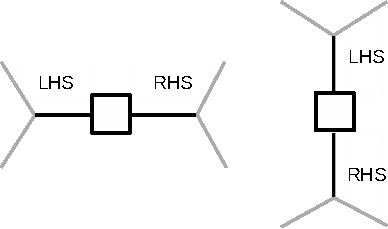
\includegraphics[scale = 0.4]{images/process_sidedness}
  \caption{An illustration of the ``sidedness'' of a process. The designation of LHS and RHS is essentially arbitrary.}
  \label{fig:process-sidedness}
\end{figure}

\subsubsection{Flux Arcs}

\begin{enumerate}
\item All process nodes (with the exception of \glyph{phenotype}) must have a LHS and RHS.
    \item All EPNs on the LHS of a process must be unique.
    \item All EPNs on the RHS of a process must be unique.
    \item All \glyph{phenotype} glyphs must be associated with at least one modulation arc.
    \item The EPNs that make up the LHS of the process should be consistent with the RHS, i.e.\, the process should constitute a    balanced biochemical reaction.
    \item Once the stoichiometry of a flux arc is displayed in a map then all other flux arcs should
    display theit stoichiometry make.
    \item If the stoichiometry is undefined or unknown this should be indicated by the use of a question mark (``?''). 
   \item If more than one set of stoichiometries can be applied to the flux arcs of the process then the stoichiometry of the flux arcs must be displayed.
%     \item \glyph{PNs} should have only one \glyph{Catalysis} arc connected to them. If
%     there more than one catalyst known to affect the process, several \glyph{PNs} should be
%     drawn or a \glyph{logical operator} used 
%     \item \glyph{PNs} should have only one \glyph{necessary stimulation} arc connected to it. If
%     there is more than one \glyph{EPN} acting as a necessary stimulator on a process, then a \glyph{logic operator} should be used.
\end{enumerate}  

\subsubsection{\glyph{Association}}

  \begin{enumerate}
    \item An \glyph{Association} is always an irreversible process.
\end{enumerate}  

\subsubsection{\glyph{Dissociation}}
  \begin{enumerate}
    \item An \glyph{Dissociation} is always an irreversible process.
\end{enumerate}  

\subsubsection{Modulation}
\label{sec:mod-semantics}

As discussed in \sect{concepts}, it is implied, but not defined explicitly that the process has a rate at
which it converts its LHS EPNs to its RHS EPNs (and vice-versa in the case of a reversible process). This concept is
important in understanding how the \PDl describes process modulation.

\begin{enumerate}
\item A \glyph{process} with no modulations has an underlying ``basal rate''
  which describes the rate at which it converts inputs to outputs.
\item A \glyph{modulation} changes the basal rate in an unspecified fashion.
\item A \glyph{stimulation} is a modulation that increases the basal rate.
\item An \glyph{inhibition} is a modulation that decreases the basal rate.
\item The above types of modulation, when assigned to the same process, are combined and have a multiplicative effect on the basal rate of the process.
\item Modulators that do not interact with each other in the above manner, should be drawn as modulating different process nodes. Their effect is therefore additive.
\item At most one \glyph{necessary stimulation} can be assigned to a process node. Two \glyph{necessary stimulations}
  would imply an implicit AND or OR operator. For clarity only
  one \glyph{necessary stimulation} can be assigned to a \glyph{process}, and such combinations must be
  explicitly expressed using \glyph{logical operators}.  \item At most one \glyph{catalysis} can be assigned to a \glyph{process}. A catalysis arcs
  modulation implies that the exact biochemical mechanism underlying
  the process is known. In this context two \glyph{catalysis} cannot
  be assigned to the same process node as they represent
  independent reactions. Other EPNs can be
  assigned to the same process than a catalysis, such as modulators, stimulators, and
  inhibitors, and will have a multiplicative modulation on the reaction
  rate defined by the catalysis.
\end{enumerate}

\subsubsection{Reversible Processes}
\label{sec: semantics reversible procs}

A process is deemed to be reversible if it has \glyph{production} arcs on both the LHS and RHS of a process node \fig{process-reversibility}. Semantically, the \glyph{production} arc can be thought of as allowing a reversible flow of entities between the \glyph{process} and the \glyph{EPN}. A \glyph{consumption} arc only permits an irreversible flow from the \glyph{EPN} to the \glyph{process}. In this way, the \glyph{consumption} arc forces the \glyph{process} to be irreversible. \glyph{Consumption} arcs cannot be associated with both sides of a \glyph{process} as this would prohibit any flow through the \glyph{process}.

\begin{figure}[H]
  \centering
  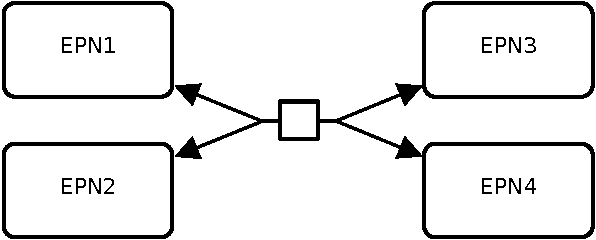
\includegraphics[scale = 0.4]{images/reversible_process}
  \caption{A valid reversible process. A process is reversible if its LHS and RHS contain only \glyph{production} arcs.}
  \label{fig:process-reversibility}
\end{figure}
 
\begin{enumerate}
\item  A mixture of \glyph{consumption} and \glyph{production} arcs on the same side of a \glyph{process} is not permitted.
\item A \glyph{sink} cannot be linked to a reversible process as it only receives entities, and so would effectively make the process irreversible\footnote{A \glyph{source} can only be associated with a \glyph{consumption} arc so this rule does not apply in this case.}.
\item The semantics of \glyph{modulation} is the same as for irreversible processes, .i.e. the amount of entity in the modulation pool affects the rate of the process.
\end{enumerate}

 
\subsection{Cloning}

SBGN allows identical nodes to be duplicated on a map if they are
explicitly marked as such. This is done using a \glyph{clone marker}. The details are shown in table \ref{tab:processduprules}.


\begin{center}
\tablecaption{Duplication rules.}
\label{tab:processduprules}
\begin{footnotesize}
\tablefirsthead{\hline
  Node & Can be duplicated & Indication & Additional Rules\\\hline}
\tablehead{\hline
\multicolumn{4}{|l|}{\small\sl continued from previous page}\\
\hline\hline
  Node & Duplicate? & Indication & Additional Rules\\\hline\hline}
\tabletail{\hline
\multicolumn{4}{|r|}{\small\sl continued on next page}\\
\hline}
\tablelasttail{\hline}
\begin{supertabular}{|l|c|p{4cm}|p{3.5cm}|}\hline
%  Node & Duplicate? & How & Additional Rules\\\hline
Compartment   & N & & \\\hline
SimpleChemical & Y & \glyph{Simple clone marker} & \\\hline
UnspecifiedEntity & Y & \glyph{Simple clone marker} & \\\hline
Source & N & & \\\hline
Sink & N & & \\\hline
Perturbing Agent & Y & \glyph{Simple clone marker} & \\\hline
Phenotype & Y & \glyph{Simple clone marker} & \\\hline
MultimerChemicalEntity & Y & \glyph{Simple clone marker} & \\\hline
StatefulEntityPool & Y & \glyph{Labeled clone marker} & \\\hline
Macromolecule & Y & \glyph{Labeled clone marker} & \\\hline
MultimerMacromolecule & Y & \glyph{Labeled clone marker} & \\\hline
Nucleic\-Acid\-Feature & Y & \glyph{Labeled clone marker} & \\\hline
Complex & Y & \glyph{Labeled clone marker} & \\\hline
Process & Y & None & Duplication is implied when all EPNs linked to the Process are marked as clones.\\\hline
OmittedProcess & Y & As Process  & \\\hline
UncertainProcess & Y & As Process  & \\\hline
Association & Y & As Process  & \\\hline
Dissociation & Y & As Process  & \\\hline
LogicalOperator & Y & None & \\\hline
AND & Y & None & \\\hline
OR & Y & None & \\\hline
NOT & Y & None & \\\hline
\end{supertabular}
\end{footnotesize}
\end{center}


\subsection{Compartment spanning}

An \glyph{EPN} cannot \emph{belong} to more than one
\glyph{compartment}. However, an EPN can be \emph{drawn} over more than one
\glyph{compartment}. In such cases, the decision on which is the owning
\glyph{compartment} is deferred to the drawing tool or the
author. A \glyph{complex} may contain EPNs which belong to different
\glyph{compartments} and in this way a \glyph{complex} can be used to describe
entities that span more than one {compartment}.

This restriction makes it impossible to represent in a semantically
correct way a macromolecule that spans more then one compartment ---
for example a receptor protein. It is clearly desirable to be able to
show a macromolecule in a manner that the biologist expects (i.e.\,
spanning from the outside through the membrane to the
inside). Therefore, the author is recommended to draw the
macromolecule across compartment boundaries, but the underlying SBGN
semantic model will assign it to only one. The assignment to a
\glyph{compartment} may be decided by the software drawing tool or the
author. Note that this has implications for auto-layout algorithms as
they will only be able to treat such \glyph{entity pool nodes} as contained within
a \glyph{compartment} and will have no way of knowing a macromolecule spans a
compartment.

The current solution is consistent with other Systems Biology
representations such as SBML and BioPAX. For more information about the
problems representing membrane spanning proteins and the rationale
behind the current solution see \sect{postponed}.

\subsection{Submaps}

The submap is a visual device that allows the detail of an \PD map to be exported into another \PD map and replaced by a \glyph{submap} glyph, which acts as a place-holder. This is described and illustrated in \sect{submap}. In the following discussion we will refer to the original map as the \emph{main} map and the map containing the export detail as the submap. 

\begin{enumerate}
\item For a valid mapping between an EPN in the map and submap to exist the identifiers in the \glyph{tag} and the submap terminal must be identical and their associated entity pool nodes must be identical.
\item If the same EPN is present in the map and a submap, then they must be mapped to each other.
\item Since the main map and submap share the same namespace, an EPN that is cloned in the main map must also be
marked as cloned in the submap --- even if there is only one copy of the EPN in the submap. The converse applies when the EPN in the submap is cloned\footnote{This has the additional benefit of ensuring that main maps and submaps do not need to be modified if the submap is exanded and collapsed by a viewing or editing tool.}.
\end{enumerate}

% \section{Summary of Rules}

% This section summarises the rules of SBGN-PD in a form that is intended to be accessible to tool developers and those interested in validating process maps. Each rule has been given an identifier for ease of reference. Note that no meaning is attached to the rule identifier and any perceived ordering of the identifiers is not significant.

% \subsection{Entity Pool Nodes}

% \begin{description}
% \item[PD1] The identity of an EPN is defined by a combination of its compartment, entity type (e.g. complex or macromolecule), name and state variables (if any).
% \item[PD2] A Complex’s identity consists of the identity of its subunits and a name is optional. All complexes with the same name should have the same subunits.
% \item[PD3] An EPN may belong to only one compartment.
% \item[PD4] An EPN belongs to only one compartment. If no compartment is draw it is assumed to belong to a “default” compartment.
% \item[PD5] An EPN can overlap more than one compartment and in this case it is deferred to the drawing tool or author to assign the owning compartment. Note this rule need not apply in cases where SBGN is draw by hand.
% \item[PD6] A Complex may contain subunits that belong to different compartments (the complex itself will belong to only one, however).
% \item[PD7] The layout or organisation of a compartment does not imply anything about its topology.
% \item[PD8] The layout or organisation of the EPNs in a complex does not imply any information about topology.
% \item[PD10] Complexes can be nested. This does imply information about the complex’s topology.
% \item[PD11] A complex should consist of different EPNs. If two or more elements of the complex are identical then they should be replaced by a multimer.
% \item[PD12] Source and sink nodes must have no name and be attached to only one consumption or production arc.
% \item[PD13] An EPN must be connected to at least 1 consumption, production or modulation arc.
% \item[PD14] An EPN is not allowed to be a substrate and product of the same process. This applies to cloned EPNs as well.
% States
% \item[PD15] All state variables in a stateful EPN should have different names.
% \item[PD16] A blank state variable has the value “unset”.
% \item[PD17] The state of a complex is the sum of its subunits’ and its own state variables.
% \item[PD48] The \glyph{Sink} cannot be linked to a reversible process.
% \end{description}

% \subsection{Compartments}

% \begin{description}
% \item[PD18] Compartments cannot be nested. Compartments may overlap, but overlap does not imply containment.
% \item[PD19] The layout or organisation of a compartment does not imply anything about its topology.
% \item[PD20] If no compartment is draw it is assumed to belong to a “default” compartment.
% \item[PD21] If one or more compartment glyphs are drawn then all EPNs must owned by a compartment glyph.
% \end{description}

% \subsection{Process Nodes (PN)}

% \begin{description}
% \item[PD22] A Process Node should have non-zero number of consumption and production links.
% \item[PD23] All substrates of the Process Node should be different. If several copies of the same EPN are involved in the process, the cardinality label of consumption arc should be used.
% \item[PD24] All products of the PN should be different. If several copies of the same EPN are produced in the process, the cardinality label of production arc should be used.
% \item[PD25] Once the cardinality label is added to one arc connected to a PN all other such arcs should display a cardinality label.
% \item[PD26] The cardinality of an arc can be undefined or unknown, in which case a question mark (``?'') should be used.
% \item[PD27] A PN should correspond to only one process or series of connected process. The same set of EPNs should be connected by different PNs if they are consumed and produced by different processes.
% \item[PD28] The composition of the products of an association process should be equivalent to its substrates
% \item[PD29] The composition of the products of a dissociation process should be equivalent to its substrate.
% \end{description}

% \subsection{Modulation and Logical Operators}

% \begin{description}
% \item[PD30] A PN with no modulations has an underlying “basal rate” which describes the rate at which it converts inputs to outputs.
% \item[PD31] Modulation changes the basal rate in an unspecified fashion.
% \item[PD32] Stimulation is a modulation that’s effect is to increase the basal rate.
% \item[PD33] Inhibition is a modulation that’s effect is to decrease the basal rate.
% \item[PD34] The above types of modulation, when assigned to the same process are combined and have a multiplicative effect on the basal rate of the process.
% \item[PD35] Modulators that do not interact with each other in the above manner should be drawn as modulating different process nodes. Their effect is therefore additive.
% \item[PD36] At most one trigger can be assigned to a process. Two triggers would imply an implicit Boolean AND or OR operator, so for clarity only one trigger can be assigned to a process and such combinations must be explicitly expressed as the Boolean operators.
% \item[PD37] The PN should have only one Catalysis arc connected to it. A catalysis modulation implies that the exact biochemical mechanism underlying the process is known.
% \item[PD38] The PN should have only one Trigger arc connected to it.
% \item[PD39] AND and OR Boolean logic gates should have two or more input and one output.
% \item[PD40] A NOT gate can only have one input and output.
% \end{description}

% \subsection{Cloning and Sub-Maps}

% \begin{description}
% \item[PD41] Duplicate EPNs must be marked as clones.
% \item[PD42] Duplicate stateful EPNs must use a Labelled Clone Marker.
% \item[PD43] Duplicate non-stateful EPNs must use a simple clone marker.
% \item[PD44] A sub-map shares the same namespace as its main map.
% \item[PD45] To map an EPN in the main map to one in a sub-map, the SubMap glyph in the main map must contain an identifier that matches the identifier of a Tag in the sub-map. Both EPNs must be identical.
% \item[PD46] If a main map and a sub-map contain an identical EPN then a mapping must exist between them.
% \item[PD47] If an EPN is cloned in the main map, then it must be marked as cloned in the sub-map, with the same identifier in both maps. This is true if there is only one EPN of this type in the submap.
% \end{description}


